\lettrine{T}{he} Policy Evaluation Algorithm ~\ref{definition:policy-evaluation} is applied to a specific identity, and the final evaluation is the process to assess multiple policies at runtime. 

\vspace{15pt}

This approach is highly flexible as it allows writing, composing, and evaluating policies. 
However, it poses a risk, as introducing a new policy could potentially expose the system to high risks. Therefore, it is crucial to define an approach that would calculate a risk score for each of the existing identities.

\vspace{15pt}

As depicted in Figure ~\ref{fig:risk-score-policy-structure}, a policy can be described as a triple, consisting of the following components:

\begin{itemize}
    \item \textbf{Effect}: The effect of the policy can be either $ALLOW$ or $DENY$
    \item \textbf{Resource}: The resource target of the action to be performed
    \item \textbf{Action}: The action to be performed.
\end{itemize}

\begin{figure}[h]
    \centering
    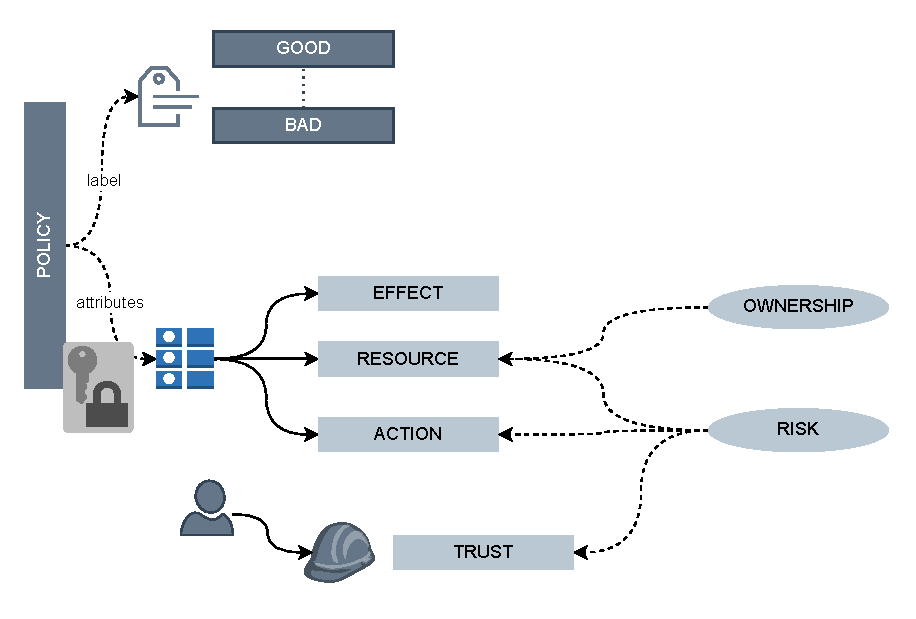
\includegraphics[width=\linewidth]{generated-risk-scores/risk-score-policy-structure.pdf}
    \caption{Policy Risk Score Structure}
    \label{fig:risk-score-policy-structure}
\end{figure}

Policies in the context of identity association can be further augmented with the following concepts:
\begin{itemize}
    \item \textbf{Ownership}: A  resource incorporates the concept of ownership, which in a multi-tenant context can be detailed as:
    \begin{itemize}
        \item \textbf{Platform}: The owner of the software solution
        \item \textbf{Tenant}: A tenant configured within the platform
        \item \textbf{User}: A user registered within the platform.
        \item \textbf{External}: An external resource, representing a third-party system that is integrated.
     \end{itemize}
    \item \textbf{Trust}: This reflects the level of trust that the platform owner places in the specific type of identity
    \item \textbf{Risk}: Risk is a value ranging from $0$ to $1$, indicating the level of risk associated with a resource, action, or trust.
\end{itemize}

\vspace{15pt}

To assign a risk score to each identity, the proposed solution leverages a Machine Learning approach that assigns a score to a sample of policies and subsequently constructs a machine learning model. 
Establishing a procedure to create the dataset for building the machine learning model is essential.

\begin{table*}[htbp]
    \caption{Policy Risk Score Input}
    \label{table:table-policy-risk-score}
    \begin{center}
    \begin{tabular}{|c|c|c|c|c|c|c|c|}
    \hline
    Effect & Res. Ownership & Res. Legal Risk & Res. Revenue Risk & Res. Reputational Risk & Action Risk &  Action Operation & Identity Trust Risk \\
    \hline
    allow & TENANT & 1 & 0.8 & 0.7 & 0.8 & DELETE & 0.3\\
    \hline
    deny & USER & 0.4 & 0.3 & 0.4 & 0.7 & PUT & 0.5\\
    \hline
    allow & TENANT & 1 & 0.9 & 0.8 & 0.2 & GET & 0.4\\
    \hline
    allow & PLATFORM & 1 & 0.9 & 0.8 & 0.2 & POST & 0.4\\
    \hline
    \end{tabular}
    \end{center}
\end{table*}

Initially, the collection of all policies associated with the identity under assessment is required. 
For each policy, the creation of a Policy Risk Score Input rapresentation is mandatory, defined as follows:
\begin{itemize}
    \item \textbf{Effect}: The effect of the policy can be either $ALLOW$ or $DENY$
    \item \textbf{Resource Ownership}: Owner of the resource. The domain is a set that includes the following values: $PLATFORM$, $TENANT$, $USER$, $EXTERNAL$
    \item \textbf{Resource Legal Risk}: Risk based on legal repercussions in the event of a security breach. The domain is \( x \in \mathbb{R}, \ 0 \leq x \leq 1 \)
    \item \textbf{Resource Revenue Risk}: Risk based on revenue repercussions in the event of a security breach. The domain is \( x \in \mathbb{R}, \ 0 \leq x \leq 1 \)
    \item \textbf{Resource Reputational Risk}: Risk based on reputational repercussions in the event of a security breach. The domain is \( x \in \mathbb{R}, \ 0 \leq x \leq 1 \)
    \item \textbf{Action Risk}: Risk based on how the action can alter the system. The domain is \( x \in \mathbb{R}, \ 0 \leq x \leq 1 \)
    \item \textbf{Action Operation}: Type of operation. The domain is a set that contains the following value: $GET$, $POST$, $PUT$, $PATCH$, $DELETE$, $SOFTDELETE$
    \item \textbf{Identity Trust Risk}: Risks based on the trust in the type of identity. The domain is \( x \in \mathbb{R}, \ 0 \leq x \leq 1 \).
\end{itemize}

\vspace{15pt}

The values used to form the Policy Risk Score Input are assigned to each resource and action during the system configuration by developers. 
Subsequently, these values are employed to construct the Policy Risk Score Input.

\vspace{15pt}

Let's define $PRISK$ as the set containing a Policy Risk Score Input representation for each policy assigned to an identity. Each item belonging to $PRISK$ is associated with a score that can range between values classified as either $GOOD$ or $BAD$.
The domain is \( x \in \mathbb{R}, \ 0 \leq x \leq 1 \).

\vspace{15pt}

A dataset is constructed by selecting n identities and creating for each of them a $PRISK$ set associated with a risk score. 
Once the dataset has been built, it is necessary to construct a machine learning model that learns from the dataset and predicts the risk of a given identity.

\vspace{15pt}

The focus of this paper is to build the dataset; however, constructing the machine learning model is beyond the scope of this document. Ideally, it would be necessary to create multiple machine learning models and compare them to find the one that fits best.

\vspace{15pt}

This approach can be further extended through the use of ontologies. Developers configure resources and actions with values utilized to create the Policy Risk Score Input representation and then building the Machine Learning model.

When tackling a new business domain, it would be possible to create an ontology that maps the new domain and establishes links with the ontology of the initial configured domain. 
This would facilitate the inference of values for the resources and actions of the new business domain, and, more importantly, it would allow the utilization of the Machine Learning model to assess the new domain.

\begin{figure}[h]
    \centering
    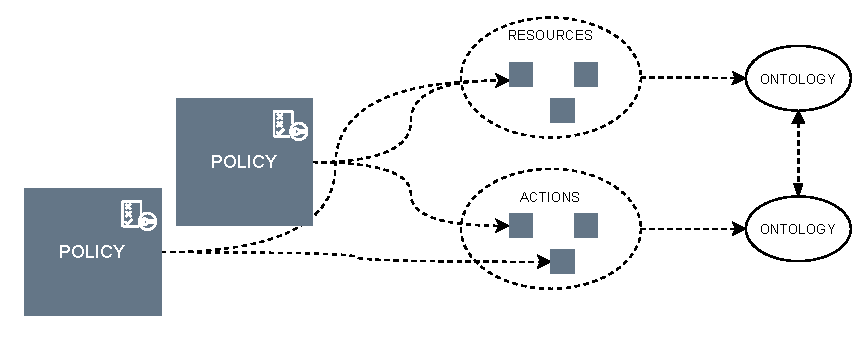
\includegraphics[width=\linewidth]{generated-risk-scores/ontology-mapping.pdf}
    \caption{Ontology Mapping}
    \label{fig:ontology-mapping}
\end{figure}.